\documentclass[11pt]{article}

\usepackage[margin=1in]{geometry}
\usepackage{amsmath,amssymb,mathtools}
\usepackage{booktabs}
\usepackage{float}
\usepackage{graphicx}
\usepackage{microtype}
\usepackage[round]{natbib}
\usepackage{tabularx}
\usepackage{enumitem}
\usepackage{xcolor}
\usepackage{hyperref}
\usepackage{tikz}
\usetikzlibrary{arrows.meta,positioning,calc}

\hypersetup{
  colorlinks=true,
  linkcolor=blue!55!black,
  citecolor=blue!55!black,
  urlcolor=blue!55!black,
}

\setlist[itemize]{leftmargin=*,itemsep=0.25em,topsep=0.4em}
\setlength{\parindent}{0pt}
\setlength{\parskip}{0.55em}
\renewcommand{\arraystretch}{1.18}

\newcommand{\R}{\mathbb{R}}
\newcommand{\softmax}{\operatorname{softmax}}
\newcommand{\TopK}{\operatorname{TopK}}
\newcommand{\RMSNorm}{\operatorname{RMSNorm}}
\newcommand{\LN}{\operatorname{LN}}
\newcommand{\SiLU}{\operatorname{SiLU}}

\title{Modern Transformer Architecture\\
\large Attention and Mixture of Experts}
\author{Haowu Duan}
\date{\today}

\begin{document}

\maketitle

\begin{abstract}
This note derives causal softmax attention and token-choice sparse
mixture-of-experts (MoE) layers in decoder-only Transformers.  It identifies the
hyperparameters that determine stability, memory, communication, and inference cost.
\end{abstract}

\textbf{Primary resources.}
The two major resources are the Microsoft AI technical report
\emph{MAI-Thinking-1: Building a Hill-Climbing Machine}
\citep{microsoftai2026maithinking} and Lectures 3 and 4 of Stanford's CS336,
\emph{Language Modeling from Scratch}, taught by Tatsunori Hashimoto
\citep{hashimoto2026architecture,hashimoto2026attentionmoe}.  The MAI report supplies
the reference architecture; the Stanford lectures supply the hyperparameter framing.
Original papers are cited for individual methods.

\vspace{1em}
\noindent\fbox{%
  \parbox{0.94\textwidth}{%
  \textbf{Scope.} Included: causal softmax attention, normalization and residual
  placement, the dense FFN baseline, token-choice sparse MoE, and selected evidence
  needed to explain why MoE is used.  Excluded: linear attention, full model catalogs,
  comprehensive routing surveys, and detailed ablations.}}

\clearpage
\tableofcontents
\clearpage

% =====================================================================
\section{Attention}
% =====================================================================

\subsection{One causal attention head}

The batch size is $B$, and $b\in\{1,\ldots,B\}$ labels one batch element.
A token sequence is a one-dimensional lattice with sites
$i=1,\ldots,S$.  At site $i$, the token is represented by a vector
$e_i^{(b)}\in\R^{d_{\mathrm{model}}}$.  With additive positional encoding, a
position vector $p_i\in\R^{d_{\mathrm{model}}}$ is added at the same site:
\begin{equation}
  x_i^{(b)}=e_i^{(b)}+p_i,
  \qquad
  x_i^{(b)}\in\R^{d_{\mathrm{model}}}.
  \label{eq:additive-position}
\end{equation}
Stacking the site vectors gives
$X^{(b)}\in\R^{S\times d_{\mathrm{model}}}$.

\begin{figure}[H]
  \centering
  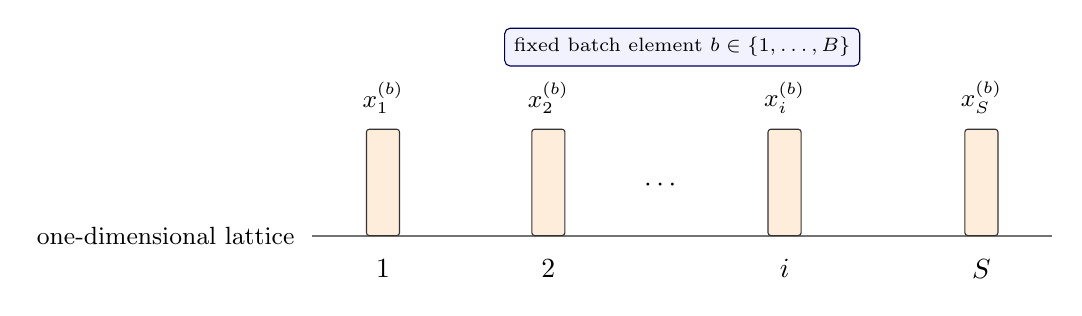
\begin{tikzpicture}[
    statevec/.style={draw=black!80,fill=orange!14,rounded corners=1pt,
      minimum width=0.42cm,minimum height=1.35cm,inner sep=0pt},
    veclabel/.style={font=\small,align=center}
  ]
    \node[draw=blue!35!black,fill=blue!5,rounded corners=2pt,
      font=\scriptsize] at (4.7,3.65)
      {fixed batch element $b\in\{1,\ldots,B\}$};

    \draw[thick,black!55] (0,1.25) -- (9.4,1.25);
    \node[statevec,anchor=south] (x1) at (0.9,1.25) {};
    \node[statevec,anchor=south] (x2) at (3.0,1.25) {};
    \node at (4.45,1.9) {$\cdots$};
    \node[statevec,anchor=south] (xi) at (6.0,1.25) {};
    \node[statevec,anchor=south] (xS) at (8.5,1.25) {};
    \node[veclabel,above=2pt of x1] {$x_1^{(b)}$};
    \node[veclabel,above=2pt of x2] {$x_2^{(b)}$};
    \node[veclabel,above=2pt of xi] {$x_i^{(b)}$};
    \node[veclabel,above=2pt of xS] {$x_S^{(b)}$};
    \node[below=5pt] at (0.9,1.25) {$1$};
    \node[below=5pt] at (3.0,1.25) {$2$};
    \node[below=5pt] at (6.0,1.25) {$i$};
    \node[below=5pt] at (8.5,1.25) {$S$};
    \node[anchor=east,font=\small] at (-0.1,1.25)
      {one-dimensional lattice};
  \end{tikzpicture}
  \caption{A sequence as a one-dimensional lattice.  Each site carries one
  $d_{\mathrm{model}}$-component vector.}
  \label{fig:token-lattice}
\end{figure}

Equation~\eqref{eq:additive-position} is additive positional encoding.  RoPE instead
rotates projected queries and keys; see Section~\ref{sec:multihead}.

An attention head maps three matrices $Q,K,V$ to one matrix $H$.  For one head
of width $d_h$, the projection matrices are
\[
  W_Q,W_K,W_V\in\R^{d_{\mathrm{model}}\times d_h}
\]
and define
\begin{align}
  Q_{im}^{(b)}
  &=\sum_{r=1}^{d_{\mathrm{model}}}X_{ir}^{(b)}(W_Q)_{rm},
  &Q^{(b)}&\in\R^{S\times d_h},\\
  K_{jm}^{(b)}
  &=\sum_{r=1}^{d_{\mathrm{model}}}X_{jr}^{(b)}(W_K)_{rm},
  &K^{(b)}&\in\R^{S\times d_h},\\
  V_{jm}^{(b)}
  &=\sum_{r=1}^{d_{\mathrm{model}}}X_{jr}^{(b)}(W_V)_{rm},
  &V^{(b)}&\in\R^{S\times d_h}.
\end{align}
\clearpage
For the rest of the one-head calculation, fix $b$ and suppress its label, so
$Q,K,V\in\R^{S\times d_h}$.
Their $i$th rows, $q_i$, $k_i$, and $v_i$, are the query, key, and value at
token position $i$.  The head output is obtained in four steps:
\begin{align}
  A_{ij}
  &=\frac{1}{\sqrt{d_h}}
    \sum_{m=1}^{d_h}Q_{im}(K^{\mathsf T})_{mj},
  \label{eq:one-head-score}\\
  \Lambda_{ij}
  &=A_{ij}+M_{ij},
  \label{eq:one-head-logit}\\
  P_{ij}
  &=\frac{\exp(\Lambda_{ij})}
    {\sum_{j'=1}^{S}\exp(\Lambda_{ij'})},
  \label{eq:one-head-probability}\\
  H_{im}
  &=\sum_{j=1}^{S}P_{ij}V_{jm}.
  \label{eq:one-head-output}
\end{align}
Here $(K^{\mathsf T})_{mj}=K_{jm}$,
$A,\Lambda,P\in\R^{S\times S}$, and $H\in\R^{S\times d_h}$.  The notation is:
\begin{center}
\small
\begin{tabular}{@{}c l@{}}
$A_{ij}$ & scaled \emph{attention score} before masking, \\
$\Lambda_{ij}$ & masked \emph{attention logit} passed to softmax, \\
$P_{ij}$ & normalized \emph{attention weight} (or attention probability). \\
\end{tabular}
\end{center}
For a causal head,
\[
  M_{ij}=\begin{cases}
    0, & j\le i,\\
    -\infty, & j>i.
  \end{cases}
\]
Therefore $P_{ij}=0$ when $j>i$.  For fixed $i$, the remaining $P_{ij}$ are
non-negative and sum to one, so $H_i$ is a weighted average of the current and
earlier value vectors.  This is causal self-attention.

The head width $d_h$ does not have to equal $d_{\mathrm{model}}$.  Restoring
the batch label, the output projection
\begin{equation}
  \mathcal{A}(X^{(b)})=H^{(b)}W_O
  \in\R^{S\times d_{\mathrm{model}}},
  \qquad
  W_O\in\R^{d_h\times d_{\mathrm{model}}}
\end{equation}
maps the head output back to the residual-stream width.

\subsection{From one head to multiple heads}
\label{sec:multihead}

A multi-head layer contains $n_q$ query heads, labelled
$h\in\{1,\ldots,n_q\}$.  The head label is written as a superscript.  For the
fixed batch element $b$, the input to the attention layer is
$Z^{(b)}\in\R^{S\times d_{\mathrm{model}}}$.  The index
$r\in\{1,\ldots,d_{\mathrm{model}}\}$ labels an input component, and
$m\in\{1,\ldots,d_h\}$ labels a component within one head.  In ordinary
multi-head attention, head $h$ has projection matrices
\[
  W_Q^{(h)},W_K^{(h)},W_V^{(h)}
  \in\R^{d_{\mathrm{model}}\times d_h}.
\]
They produce
\begin{align}
  Q_{im}^{(b,h)}
  &=\sum_{r=1}^{d_{\mathrm{model}}}
    Z_{ir}^{(b)}(W_Q^{(h)})_{rm},
  &Q^{(b,h)}&\in\R^{S\times d_h},\\
  K_{jm}^{(b,h)}
  &=\sum_{r=1}^{d_{\mathrm{model}}}
    Z_{jr}^{(b)}(W_K^{(h)})_{rm},
  &K^{(b,h)}&\in\R^{S\times d_h},\\
  V_{jm}^{(b,h)}
  &=\sum_{r=1}^{d_{\mathrm{model}}}
    Z_{jr}^{(b)}(W_V^{(h)})_{rm},
  &V^{(b,h)}&\in\R^{S\times d_h}.
\end{align}
The sum contracts the input index $r$.  The head label $h$ is not summed: it
specifies which projection matrix is used.

The one-head calculation is applied separately for every $h$:
\begin{align}
  A_{ij}^{(b,h)}
  &=\frac{1}{\sqrt{d_h}}
    \sum_{m=1}^{d_h}Q_{im}^{(b,h)}
    \bigl((K^{(b,h)})^{\mathsf T}\bigr)_{mj},
  \label{eq:attention-score}\\
  \Lambda_{ij}^{(b,h)}
  &=A_{ij}^{(b,h)}+M_{ij},
  \label{eq:attention-logit}\\
  P_{ij}^{(b,h)}
  &=\frac{\exp(\Lambda_{ij}^{(b,h)})}
    {\sum_{j'=1}^{S}\exp(\Lambda_{ij'}^{(b,h)})},
  \label{eq:attention-probability}\\
  H_{im}^{(b,h)}
  &=\sum_{j=1}^{S}P_{ij}^{(b,h)}V_{jm}^{(b,h)}.
  \label{eq:attention}
\end{align}
Since $\bigl((K^{(b,h)})^{\mathsf T}\bigr)_{mj}=K_{jm}^{(b,h)}$, each head
produces $H^{(b,h)}\in\R^{S\times d_h}$.  Placing the outputs side by side gives
\begin{equation}
  H_{\mathrm{cat}}^{(b)}
  =\bigl[H^{(b,1)}\mid\cdots\mid H^{(b,n_q)}\bigr]
  \in\R^{S\times(n_qd_h)}.
\end{equation}
The output projection returns to the residual-stream width:
\begin{equation}
  \mathcal{A}(Z^{(b)})=H_{\mathrm{cat}}^{(b)}W_O
  \in\R^{S\times d_{\mathrm{model}}},
  \qquad
  W_O\in\R^{(n_qd_h)\times d_{\mathrm{model}}}.
\end{equation}

The combined head width $n_qd_h$ does not have to equal
$d_{\mathrm{model}}$.  Most models nevertheless use
\begin{equation}
  \rho_{\mathrm{head}}=\frac{n_qd_h}{d_{\mathrm{model}}}\simeq 1.
\end{equation}
Placing the query projections side by side gives
\[
  W_Q^{\mathrm{flat}}
  =\bigl[W_Q^{(1)}\mid\cdots\mid W_Q^{(n_q)}\bigr]
  \in\R^{d_{\mathrm{model}}\times(n_qd_h)}.
\]
One matrix product computes all query heads:
\begin{equation}
  \underbrace{Z^{(b)}}_{S\times d_{\mathrm{model}}}
  \cdot
  \underbrace{W_Q^{\mathrm{flat}}}_{d_{\mathrm{model}}\times(n_qd_h)}
  =
  \underbrace{Q_{\mathrm{flat}}^{(b)}}_{S\times(n_qd_h)}
  \label{eq:query-projection-reshape}
\end{equation}
The $h$th block of $d_h$ columns in $Q_{\mathrm{flat}}^{(b)}$ is
$Q^{(b,h)}$.  Even when $\rho_{\mathrm{head}}=1$ makes
$W_Q^{\mathrm{flat}}$ square, each output component is a linear combination of
all $d_{\mathrm{model}}$ input components.

\begin{center}
\fbox{%
\begin{minipage}{0.92\textwidth}
\textbf{Rotary position embedding (RoPE).}
The positional calculation below concerns the raw query--key compatibility
$C_{ij}=q_i^{\mathsf T}k_j$.  Under the convention above, its scaled attention
score and masked attention logit are
$A_{ij}=C_{ij}/\sqrt{d_h}$ and $\Lambda_{ij}=A_{ij}+M_{ij}$.

Without a positional operation, an identical token vector produces the same query
and key at every site, so the site does not enter $C_{ij}$.  The required positional
variable for the pair $(i,j)$ is their relative displacement $j-i$.

With direct additive positional encoding, the vector entering the projection
at position $i$ is $e_i+p_i$.  For one head, suppress the batch and head labels
and write
\[
  q_i=W_Q^{\mathsf T}e_i,\qquad \pi_i^Q=W_Q^{\mathsf T}p_i,
  \qquad
  k_j=W_K^{\mathsf T}e_j,\qquad \pi_j^K=W_K^{\mathsf T}p_j.
\]
The raw compatibility is
\begin{align*}
  C_{ij}^{\mathrm{add}}
  &=(q_i+\pi_i^Q)^{\mathsf T}(k_j+\pi_j^K)\\
  &=\underbrace{q_i^{\mathsf T}k_j}_{\text{content--content}}
   +\underbrace{q_i^{\mathsf T}\pi_j^K
   +(\pi_i^Q)^{\mathsf T}k_j}_{\text{content--position cross terms}}
   +\underbrace{(\pi_i^Q)^{\mathsf T}\pi_j^K}_{\text{position--position}}.
\end{align*}
The cross terms depend separately on $i$ and $j$, not on $j-i$.  They are wasted
for encoding relative position.

RoPE instead rotates the content projections after projection and before their
dot product \citep{su2021roformer}.  For $q_i,k_j\in\R^{d_h}$,
\[
  C_{ij}^{\mathrm{RoPE}}
  =(R_iq_i)^{\mathsf T}(R_jk_j)
  =q_i^{\mathsf T}R_i^{\mathsf T}R_jk_j
  =q_i^{\mathsf T}R_{j-i}k_j.
\]
Position enters only through $j-i$; no additive content--position cross terms
appear.  The RoPE hyperparameters are the rotary dimension
$d_{\mathrm{rope}}\le d_h$, frequency base $\theta$, length-rescaling rule, and
the layers where it is applied.
\end{minipage}%
}
\end{center}

\subsection{Attention inside a decoder block}

The decoder contains $L$ blocks, indexed by
$\ell\in\{0,\ldots,L-1\}$.  For the fixed batch element $b$, the residual stream
at layer $\ell$ is $X_\ell^{(b)}\in\R^{S\times d_{\mathrm{model}}}$, where $S$ is
the number of token positions and $d_{\mathrm{model}}$ is the model width.  A
standard serial, pre-normalized decoder block acts independently on each batch element
\citep{vaswani2017attention}:
\begin{align}
  U_\ell^{(b)}
  &= X_\ell^{(b)}
   + \mathcal{A}_\ell\!\left(N_{\ell}^{\mathrm{attn}}(X_\ell^{(b)})\right),
  \label{eq:attn-residual}
  \\
  X_{\ell+1}^{(b)}
  &= U_\ell^{(b)}
   + \mathcal{F}_\ell\!\left(N_{\ell}^{\mathrm{ffn}}(U_\ell^{(b)})\right),
  \label{eq:ffn-residual}
\end{align}

\begin{figure}[H]
  \centering
  \resizebox{0.98\linewidth}{!}{%
  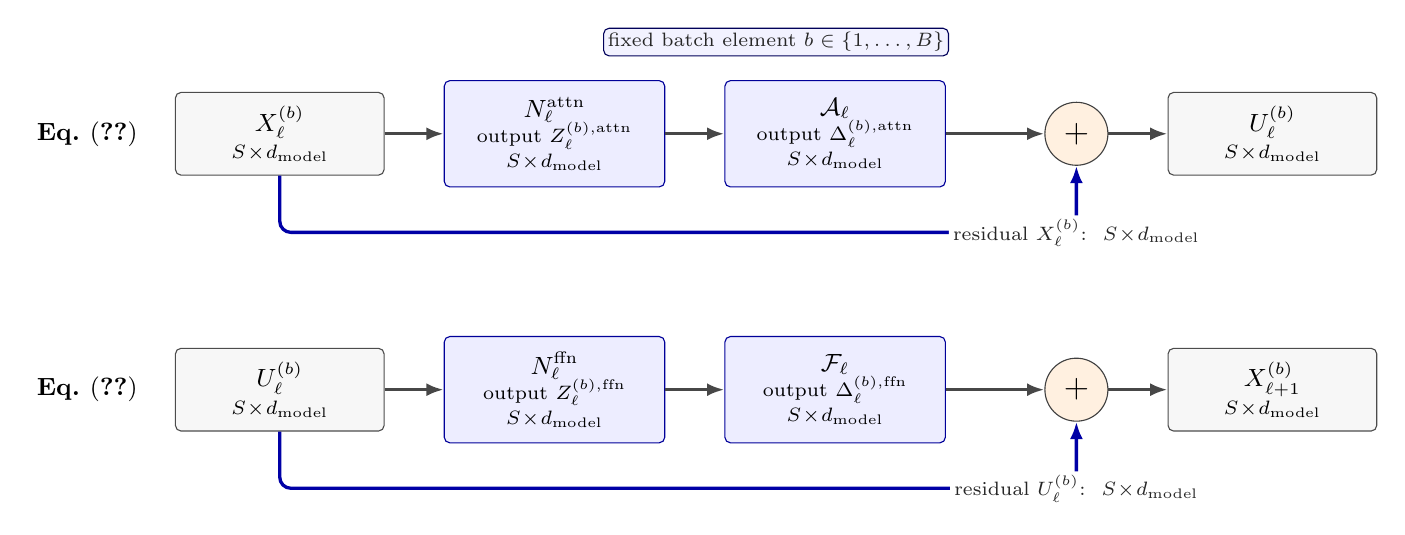
\begin{tikzpicture}[
    >={Latex[length=2.2mm]},
    flow/.style={->,very thick,draw=black!72},
    residual/.style={->,very thick,draw=blue!65!black,rounded corners=4pt},
    tensor/.style={draw=black!70,fill=black!3,rounded corners=2pt,
      minimum width=2.65cm,minimum height=1.05cm,align=center,font=\small},
    operation/.style={draw=blue!60!black,fill=blue!7,rounded corners=2pt,
      minimum width=2.8cm,minimum height=1.35cm,align=center,font=\small},
    add/.style={circle,draw=black!75,fill=orange!12,minimum size=8mm,
      inner sep=0pt,font=\large},
    quantity/.style={align=center,font=\scriptsize,text=black!85,
      fill=white,inner sep=1.5pt},
    eqlabel/.style={font=\bfseries\small,anchor=east}
  ]
    % Equation (1): attention residual update.
    \node[eqlabel] (eq1) at (-0.35,0) {Eq.~\eqref{eq:attn-residual}};
    \node[tensor,right=0.35cm of eq1] (x) {$X_\ell^{(b)}$\\[-1pt]
      {\scriptsize $S\!\times\!d_{\mathrm{model}}$}};
    \node[operation,right=0.75cm of x] (nattn) {$N_\ell^{\mathrm{attn}}$\\[-2pt]
      {\scriptsize output $Z_\ell^{(b),\mathrm{attn}}$}\\[-2pt]
      {\scriptsize $S\!\times\!d_{\mathrm{model}}$}};
    \node[operation,right=0.75cm of nattn] (attn) {$\mathcal{A}_\ell$\\[-2pt]
      {\scriptsize output $\Delta_\ell^{(b),\mathrm{attn}}$}\\[-2pt]
      {\scriptsize $S\!\times\!d_{\mathrm{model}}$}};
    \node[add,right=1.25cm of attn] (add1) {$+$};
    \node[tensor,right=0.75cm of add1] (u) {$U_\ell^{(b)}$\\[-1pt]
      {\scriptsize $S\!\times\!d_{\mathrm{model}}$}};
    \node[quantity,anchor=south,fill=blue!5,draw=blue!35!black,
      rounded corners=2pt] at ($(x.north)!0.5!(u.north)+(0,0.45)$)
      {fixed batch element $b\in\{1,\ldots,B\}$};

    \draw[flow] (x) -- (nattn);
    \draw[flow] (nattn) -- (attn);
    \draw[flow] (attn) -- (add1);
    \draw[flow] (add1) -- (u);
    \draw[residual] (x.south) -- ++(0,-0.72) -|
      node[quantity,pos=0.64,below] {residual $X_\ell^{(b)}$:\;
      $S\!\times\!d_{\mathrm{model}}$} (add1.south);

    % Equation (2): FFN/MoE residual update.
    \node[eqlabel] (eq2) at (-0.35,-3.25) {Eq.~\eqref{eq:ffn-residual}};
    \node[tensor,right=0.35cm of eq2] (uin) {$U_\ell^{(b)}$\\[-1pt]
      {\scriptsize $S\!\times\!d_{\mathrm{model}}$}};
    \node[operation,right=0.75cm of uin] (nffn) {$N_\ell^{\mathrm{ffn}}$\\[-2pt]
      {\scriptsize output $Z_\ell^{(b),\mathrm{ffn}}$}\\[-2pt]
      {\scriptsize $S\!\times\!d_{\mathrm{model}}$}};
    \node[operation,right=0.75cm of nffn] (ffn) {$\mathcal{F}_\ell$\\[-2pt]
      {\scriptsize output $\Delta_\ell^{(b),\mathrm{ffn}}$}\\[-2pt]
      {\scriptsize $S\!\times\!d_{\mathrm{model}}$}};
    \node[add,right=1.25cm of ffn] (add2) {$+$};
    \node[tensor,right=0.75cm of add2] (xnext) {$X_{\ell+1}^{(b)}$\\[-1pt]
      {\scriptsize $S\!\times\!d_{\mathrm{model}}$}};

    \draw[flow] (uin) -- (nffn);
    \draw[flow] (nffn) -- (ffn);
    \draw[flow] (ffn) -- (add2);
    \draw[flow] (add2) -- (xnext);
    \draw[residual] (uin.south) -- ++(0,-0.72) -|
      node[quantity,pos=0.64,below] {residual $U_\ell^{(b)}$:\;
      $S\!\times\!d_{\mathrm{model}}$} (add2.south);
  \end{tikzpicture}%
  }
  \caption{Dataflow for Equations~\eqref{eq:attn-residual}
  and~\eqref{eq:ffn-residual} for a fixed batch element $b$.  Black arrows follow
  the transformed branch; blue arrows are the untouched residual paths.  Each
  displayed tensor has shape $S\times d_{\mathrm{model}}$; stacking
  $b=1,\ldots,B$ gives the full-batch shape
  $B\times S\times d_{\mathrm{model}}$.}
  \label{fig:decoder-block-dataflow}
\end{figure}

The superscript $(b)$ is a batch label.  Within one batch element,
$i\in\{1,\ldots,S\}$ labels position and
$r\in\{1,\ldots,d_{\mathrm{model}}\}$ labels residual coordinate, so an entry is
$(X_\ell^{(b)})_{ir}$.  Every branch returns to
$S\times d_{\mathrm{model}}$ before residual addition.

In Equations~\eqref{eq:attn-residual}--\eqref{eq:ffn-residual}, $\mathcal{A}$ is
causal self-attention, $\mathcal{F}$ is a dense FFN or MoE layer, and $N$ is
usually RMSNorm.

This is a \emph{serial} block because the FFN reads the attention-updated
$U_\ell$.  In a parallel block, both branches read $X_\ell$:
\begin{equation}
  X_{\ell+1}
  =X_\ell
  +\mathcal{A}_\ell\!\left(N_\ell(X_\ell)\right)
  +\mathcal{F}_\ell\!\left(N_\ell(X_\ell)\right).
  \label{eq:parallel-block}
\end{equation}
The parallel branches can run concurrently.  A model using this form must state
whether they share $N_\ell$ \citep{hashimoto2026architecture}.

Depth and width are separate hyperparameters.  Their commonly quoted aspect ratio is
\begin{equation}
  \rho_{\mathrm{aspect}}
  =\frac{d_{\mathrm{model}}}{L}
  \sim 100\text{--}200.
  \label{eq:model-aspect-ratio}
\end{equation}
The range is empirical.  Since block $\ell+1$ needs the output of block $\ell$,
increasing $L$ adds serial work and latency
\citep{hashimoto2026architecture}.

\subsection{Key/value heads and the KV cache}

Fix one batch element and suppress its label.  The input to the attention layer is
$Z\in\R^{S\times d_{\mathrm{model}}}$.  The numbers of key and value heads are
$n_k$ and $n_v$, respectively.  Their indices are
\[
  a\in\{1,\ldots,n_k\},
  \qquad
  c\in\{1,\ldots,n_v\}.
\]
Their projection matrices and outputs are
\begin{align}
  W_K^{(a)}&\in\R^{d_{\mathrm{model}}\times d_h},
  &K^{(a)}&=Z\cdot W_K^{(a)}\in\R^{S\times d_h},\\
  W_V^{(c)}&\in\R^{d_{\mathrm{model}}\times d_h},
  &V^{(c)}&=Z\cdot W_V^{(c)}\in\R^{S\times d_h}.
\end{align}
Standard multi-head attention (MHA), grouped-query attention (GQA), and
multi-query attention (MQA) use $n_k=n_v$ and pair $K^{(a)}$ with $V^{(a)}$.
The two matrices in a pair are not equal; they are produced by different
projections.

In MHA, $n_k=n_v=n_q$, and query head $h$ uses $K^{(h)}$ and $V^{(h)}$.
In GQA, $1<n_k=n_v<n_q$, and several query heads use the same key and value
heads.  In MQA, $n_k=n_v=1$, and every query head uses $K^{(1)}$ and
$V^{(1)}$ \citep{ainslie2023gqa}.

For example, take $n_q=8$ and $n_k=n_v=2$.  Assign query heads $1$--$4$ to
the first key and value heads, and query heads $5$--$8$ to the second.  The
attention operations are
\begin{equation}
  \begin{array}{lll}
    h=1,\ldots,4:
    &\displaystyle
      \Lambda^{(h)}=\frac{Q^{(h)}(K^{(1)})^{\mathsf T}}{\sqrt{d_h}}+M,
    &H^{(h)}=P^{(h)}V^{(1)},\\[6pt]
    h=5,\ldots,8:
    &\displaystyle
      \Lambda^{(h)}=\frac{Q^{(h)}(K^{(2)})^{\mathsf T}}{\sqrt{d_h}}+M,
    &H^{(h)}=P^{(h)}V^{(2)}.
  \end{array}
  \label{eq:kv-head-sharing}
\end{equation}

\begin{figure}[H]
  \centering
  \resizebox{0.92\linewidth}{!}{%
  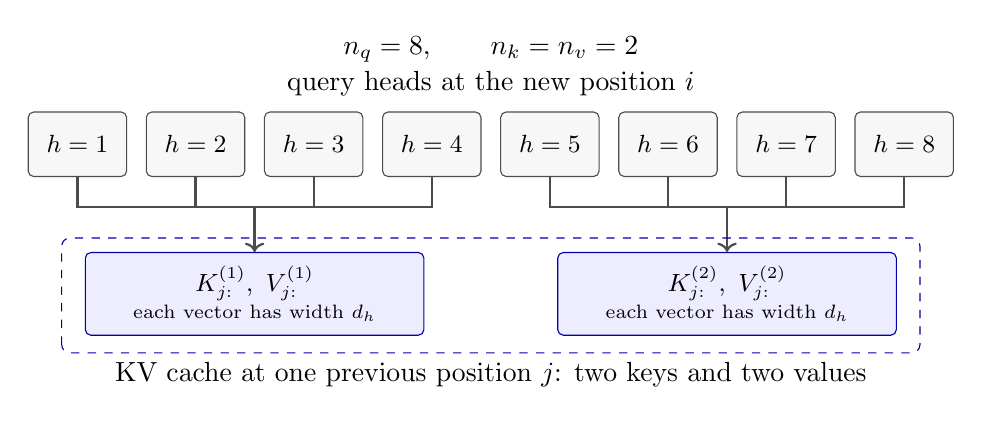
\begin{tikzpicture}[
    query/.style={draw=black!70,fill=black!3,rounded corners=2pt,
      minimum width=1.25cm,minimum height=0.82cm,align=center,font=\small},
    kv/.style={draw=blue!65!black,fill=blue!7,rounded corners=2pt,
      minimum width=4.3cm,minimum height=1.05cm,align=center,font=\small},
    group/.style={thick,draw=black!70},
    use/.style={->,thick,draw=black!70}
  ]
    \node at (0,2.55) {$n_q=8,\qquad n_k=n_v=2$};
    \node at (0,2.12) {query heads at the new position $i$};

    \foreach \h/\x in {1/-5.25,2/-3.75,3/-2.25,4/-0.75,
                         5/0.75,6/2.25,7/3.75,8/5.25} {
      \node[query] (q\h) at (\x,1.35) {$h=\h$};
    }

    \node[kv] (kv1) at (-3,-0.55)
      {$K_{j:}^{(1)},\ V_{j:}^{(1)}$\\[-1pt]
       {\scriptsize each vector has width $d_h$}};
    \node[kv] (kv2) at (3,-0.55)
      {$K_{j:}^{(2)},\ V_{j:}^{(2)}$\\[-1pt]
       {\scriptsize each vector has width $d_h$}};

    \draw[group] (-5.25,0.55) -- (-0.75,0.55);
    \draw[group] (0.75,0.55) -- (5.25,0.55);
    \foreach \h in {1,2,3,4} {\draw[group] (q\h.south) -- ++(0,-0.39);}
    \foreach \h in {5,6,7,8} {\draw[group] (q\h.south) -- ++(0,-0.39);}
    \draw[use] (-3,0.55) -- (kv1.north);
    \draw[use] (3,0.55) -- (kv2.north);

    \draw[dashed,rounded corners=3pt,draw=blue!65!black]
      (-5.45,-1.3) rectangle (5.45,0.16);
    \node at (0,-1.58) {KV cache at one previous position $j$: two keys and two values};
  \end{tikzpicture}%
  }
  \caption{GQA with $n_q=8$ and $n_k=n_v=2$.  The eight query heads remain
  distinct.  Four use the first cached key and value, and four use the second.}
  \label{fig:gqa-example}
\end{figure}

\begin{samepage}
During autoregressive inference, the prompt is known before the model runs; each
output token becomes the input used to compute the next.  This creates two phases.

\paragraph{Prefill.}
At the start of a request, the model processes all prompt positions in parallel
under the causal mask.  This one pass fills the KV cache and produces the
vocabulary logits for the first output token.

\paragraph{Decoding.}
After the first output token is selected, the model processes one new position
per step until generation stops.  Its query attends to the cache; its key and
value are appended to the cache.  The output logits select the next token.  The
query is discarded because it is not reused.

At one layer, every stored position contains $n_k$ key vectors and $n_v$ value
vectors, each with $d_h$ components.  For $B$ sequences and $S$ stored positions,
the total number of cached scalars is
\begin{equation}
  N_{\mathrm{cache}}=BS(n_k+n_v)d_h.
  \label{eq:kv-cache-count}
\end{equation}

\paragraph{Decoding speed.}
Every generated token rereads the cache.  When decoding is memory-bound, smaller
$N_{\mathrm{cache}}$ moves fewer bytes and is faster.  Sharing key and value heads
reduces $N_{\mathrm{cache}}$ \citep{hashimoto2026architecture}.
\end{samepage}

\begin{center}
\fbox{%
\begin{minipage}{0.92\textwidth}
\textbf{Speculative decoding.}
The draft model is smaller than the target model, so it decodes each token more
cheaply and supplies a candidate block $y_1,\ldots,y_m$ faster.  Since the block is known,
the target model handles it like a short prefill appended to the existing KV
cache: every layer computes $Q$, $K$, and $V$ for all $m$ positions in parallel.

The pass returns target predictions $\hat y_1,\ldots,\hat y_m$, where
$\hat y_t$ is the predicted next token after the prefix
$x,y_1,\ldots,y_{t-1}$.  Greedy verification compares $y_t$ with $\hat y_t$
token by token and accepts the longest matching prefix
\citep{leviathan2023fast}.
\end{minipage}%
}
\end{center}

\subsection{Full and sliding-window attention}

Full causal attention lets position $i$ attend to all $j\le i$.  A sliding window of
width $w$ restricts this to $i-w<j\le i$.  The cost becomes
$\mathcal{O}(Swd_h)$ per head, and the local KV history is bounded by $w$
\citep{beltagy2020longformer}.

A hybrid pattern can repeat three local layers followed by one full layer.  Each
layer type may use RoPE or no positional encoding (NoPE).  NoPE applies no
position-dependent vector, bias, or rotation; the causal mask remains
\citep{hashimoto2026architecture}.  Specify $w$, the full-layer set, each layer's
positional rule, and KV-cache eviction.  These determine receptive field and cache
memory.

\subsection{Normalization placement}

For a vector $x\in\R^D$, LayerNorm re-centers and re-scales,
\begin{equation}
  \LN(x)
  = \gamma\odot\frac{x-\mu}{\sqrt{\sigma^2+\epsilon}}+\beta,
  \qquad
  \mu=\frac{1}{D}\sum_{r=1}^{D}x_r,
  \qquad
  \sigma^2=\frac{1}{D}\sum_{r=1}^{D}(x_r-\mu)^2.
\end{equation}
RMSNorm keeps only the rescaling operation \citep{zhang2019rmsnorm}:
\begin{equation}
  \RMSNorm(x)
  = \gamma\odot
    \frac{x}{\sqrt{D^{-1}\sum_{r=1}^{D}x_r^2+\epsilon}}.
\end{equation}
RMSNorm omits mean subtraction and usually the bias $\beta$; the componentwise
gain $\gamma\in\R^D$ remains.  A bias-free Transformer also uses $y=Wx$, not
$y=Wx+b$, in attention and FFN projections.

Both norms read and write $D$ components.  LayerNorm also reduces and subtracts
the mean.  Removing those operations can make a memory-bound RMSNorm kernel faster,
although both costs are $\mathcal{O}(D)$ \citep{hashimoto2026architecture}.

An attention or FFN calculation produces an update vector, which is added to
the unchanged input vector.  Figure~\ref{fig:norm-placement} shows the three
possible positions of the normalization operation.

\begin{figure}[H]
  \centering
  \resizebox{0.96\linewidth}{!}{%
  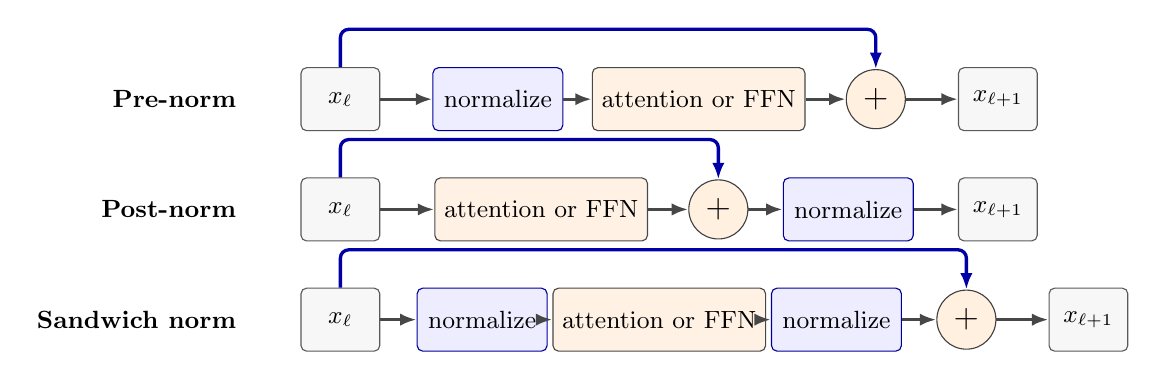
\begin{tikzpicture}[
    >={Latex[length=2.1mm]},
    flow/.style={->,very thick,draw=black!72},
    bypass/.style={->,very thick,draw=blue!65!black,rounded corners=3pt},
    vector/.style={draw=black!65,fill=black!3,rounded corners=2pt,
      minimum width=1.0cm,minimum height=0.8cm,align=center,font=\small},
    operation/.style={draw=blue!60!black,fill=blue!7,rounded corners=2pt,
      minimum width=1.65cm,minimum height=0.8cm,align=center,font=\small},
    calculation/.style={draw=black!72,fill=orange!10,rounded corners=2pt,
      minimum width=2.25cm,minimum height=0.8cm,align=center,font=\small},
    add/.style={circle,draw=black!75,fill=orange!12,minimum size=7.5mm,
      inner sep=0pt,font=\large},
    rowlabel/.style={font=\bfseries\small,anchor=east}
  ]
    \node[rowlabel] at (0,2.8) {Pre-norm};
    \node[vector] (prex) at (1.2,2.8) {$x_\ell$};
    \node[operation] (prenorm) at (3.2,2.8) {normalize};
    \node[calculation] (precalc) at (5.75,2.8) {attention or FFN};
    \node[add] (preadd) at (8.0,2.8) {$+$};
    \node[vector] (preout) at (9.55,2.8) {$x_{\ell+1}$};
    \draw[flow] (prex) -- (prenorm);
    \draw[flow] (prenorm) -- (precalc);
    \draw[flow] (precalc) -- (preadd);
    \draw[flow] (preadd) -- (preout);
    \draw[bypass] (prex.north) -- ++(0,0.48) -| (preadd.north);

    \node[rowlabel] at (0,1.4) {Post-norm};
    \node[vector] (postx) at (1.2,1.4) {$x_\ell$};
    \node[calculation] (postcalc) at (3.75,1.4) {attention or FFN};
    \node[add] (postadd) at (6.0,1.4) {$+$};
    \node[operation] (postnorm) at (7.65,1.4) {normalize};
    \node[vector] (postout) at (9.55,1.4) {$x_{\ell+1}$};
    \draw[flow] (postx) -- (postcalc);
    \draw[flow] (postcalc) -- (postadd);
    \draw[flow] (postadd) -- (postnorm);
    \draw[flow] (postnorm) -- (postout);
    \draw[bypass] (postx.north) -- ++(0,0.48) -| (postadd.north);

    \node[rowlabel] at (0,0) {Sandwich norm};
    \node[vector] (sandx) at (1.2,0) {$x_\ell$};
    \node[operation] (sandnormin) at (3.0,0) {normalize};
    \node[calculation] (sandcalc) at (5.25,0) {attention or FFN};
    \node[operation] (sandnormout) at (7.5,0) {normalize};
    \node[add] (sandadd) at (9.15,0) {$+$};
    \node[vector] (sandout) at (10.7,0) {$x_{\ell+1}$};
    \draw[flow] (sandx) -- (sandnormin);
    \draw[flow] (sandnormin) -- (sandcalc);
    \draw[flow] (sandcalc) -- (sandnormout);
    \draw[flow] (sandnormout) -- (sandadd);
    \draw[flow] (sandadd) -- (sandout);
    \draw[bypass] (sandx.north) -- ++(0,0.48) -| (sandadd.north);
  \end{tikzpicture}%
  }
  \caption{Normalization placement for one update.  The blue path carries
  $x_\ell$ unchanged to the addition.}
  \label{fig:norm-placement}
\end{figure}

At update $\ell$, $x_\ell\in\R^D$ is the input vector.  The symbol
$S_\ell(\,\cdot\,)$ denotes the attention or FFN calculation, and
$S_\ell(x_\ell)\in\R^D$ is the update vector it produces.  To see how
normalization placement behaves as depth increases, hold the placement fixed
and use it at every update, as in Figure~\ref{fig:norm-depth-stack}.  The
$S_\ell$ have different weights; only the pre-norm, post-norm, or sandwich-norm
construction is repeated.

\begin{figure}[H]
  \centering
  \resizebox{0.96\linewidth}{!}{%
  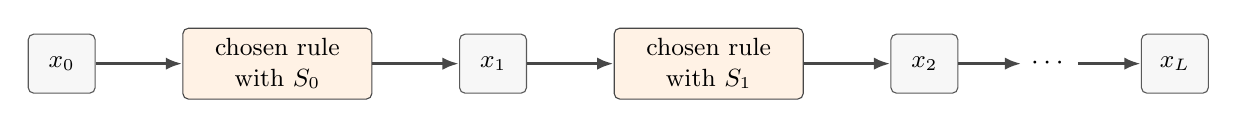
\begin{tikzpicture}[
    >={Latex[length=2.1mm]},
    flow/.style={->,very thick,draw=black!72},
    vector/.style={draw=black!65,fill=black!3,rounded corners=2pt,
      minimum width=0.85cm,minimum height=0.75cm,align=center,font=\small},
    rule/.style={draw=black!72,fill=orange!10,rounded corners=2pt,
      minimum width=2.4cm,minimum height=0.9cm,align=center,font=\small}
  ]
    \node[vector] (xzero) {$x_0$};
    \node[rule,right=1.1cm of xzero] (rulezero) {chosen rule\\with $S_0$};
    \node[vector,right=1.1cm of rulezero] (xone) {$x_1$};
    \node[rule,right=1.1cm of xone] (ruleone) {chosen rule\\with $S_1$};
    \node[vector,right=1.1cm of ruleone] (xtwo) {$x_2$};
    \node[right=0.8cm of xtwo] (dots) {$\cdots$};
    \node[vector,right=0.8cm of dots] (xlast) {$x_L$};
    \draw[flow] (xzero) -- (rulezero);
    \draw[flow] (rulezero) -- (xone);
    \draw[flow] (xone) -- (ruleone);
    \draw[flow] (ruleone) -- (xtwo);
    \draw[flow] (xtwo) -- (dots);
    \draw[flow] (dots) -- (xlast);
  \end{tikzpicture}%
  }
  \caption{Depth experiment.  The same normalization rule is used at every
  update, while $S_\ell$ has different weights at different depths.}
  \label{fig:norm-depth-stack}
\end{figure}

Repeating the normalization rule through depth changes the vector passed from
one update to the next.  Track its size with
\[
  \operatorname{rms}(v)
  \equiv\sqrt{\frac{1}{D}v^{\mathsf T}v},
  \qquad
  r_\ell\equiv\operatorname{rms}(x_\ell).
\]
In the scaling calculation below, normalization means division by this RMS;
learned gains and $\epsilon$ are suppressed.

Training sends the loss gradient backward through the same stack.  To see how
the normalization rule affects it, change the input to update $\ell$ by a
small amount $\delta x_\ell$.  To first order,
\[
  \delta x_{\ell+1}\simeq J_\ell\,\delta x_\ell,
  \qquad
  J_\ell\equiv\frac{\partial x_{\ell+1}}{\partial x_\ell}
  \in\R^{D\times D}.
\]
After the full stack in Figure~\ref{fig:norm-depth-stack},
\[
  \delta x_L
  \simeq J_{L-1}\cdots J_1J_0\,\delta x_0,
  \qquad
  \nabla_{x_0}\mathcal{L}
  =J_0^{\mathsf T}J_1^{\mathsf T}\cdots J_{L-1}^{\mathsf T}
   \nabla_{x_L}\mathcal{L}.
\]
The second equation is backpropagation through the same stack.  The product of
all layer Jacobians, rather than one $J_\ell$, therefore determines whether a
gradient is preserved, suppressed, or amplified as depth increases.

\subsubsection*{Pre-norm}
Pre-norm divides the input to $S_\ell$ by $r_\ell$:
$f_\ell=S_\ell(x_\ell/r_\ell)$.  At initialization, suppose
$\operatorname{rms}(f_\ell)\simeq s$ and
$D^{-1}x_\ell^{\mathsf T}f_\ell\simeq0$.  Then
\begin{align}
  x_{\ell+1}&=x_\ell+f_\ell,\\
  r_{\ell+1}^2
  &=r_\ell^2+s^2+\frac{2}{D}x_\ell^{\mathsf T}f_\ell
   \simeq r_\ell^2+s^2,
\end{align}
Iterating gives
\begin{equation}
  x_\ell=x_0+\sum_{k=0}^{\ell-1}f_k,
  \qquad
  r_\ell^2\simeq r_0^2+\ell s^2,
  \qquad r_\ell\sim\sqrt{\ell}.
\end{equation}
Substituting this result into the pre-norm Jacobian makes its depth dependence
explicit:
\begin{equation}
  \begin{aligned}
    J_\ell^{\mathrm{pre}}
    &=I+S_\ell'\!\left(\frac{x_\ell}{r_\ell}\right)
      \frac{1}{r_\ell}
      \left(I-\frac{x_\ell x_\ell^{\mathsf T}}{D r_\ell^2}\right)\\
    &\simeq I+
      \frac{1}{\sqrt{r_0^2+\ell s^2}}
      S_\ell'\!\left(
        \frac{x_\ell}{\sqrt{r_0^2+\ell s^2}}
      \right)
      \left(
        I-\frac{x_\ell x_\ell^{\mathsf T}}
                 {D(r_0^2+\ell s^2)}
      \right).
  \end{aligned}
  \label{eq:pre-norm-jacobian}
\end{equation}
If $S_\ell'$ does not grow with depth, then for
$\ell\gg r_0^2/s^2$, Equation~\eqref{eq:pre-norm-jacobian} further reduces to
\[
  J_\ell^{\mathrm{pre}}
  \simeq I+
  \frac{1}{s\sqrt{\ell}}
  S_\ell'\!\left(\frac{x_\ell}{s\sqrt{\ell}}\right)
  \left(I-\frac{x_\ell x_\ell^{\mathsf T}}{D\ell s^2}\right)
  =I+\mathcal{O}\!\left(\ell^{-1/2}\right).
\]
The identity $I$ gives the gradient a direct path from $x_{\ell+1}$ to
$x_\ell$.  The second term describes how layer $\ell$ changes a small input
perturbation.  The matrix in the final parentheses cannot increase a vector's
length.  The large-depth expression therefore shows directly that
$J_\ell^{\mathrm{pre}}$ approaches $I$: later layers change their inputs by a
smaller fraction and are underutilized.

\subsubsection*{Post-norm}
Post-norm first forms $u_\ell=x_\ell+S_\ell(x_\ell)$ and then divides the sum
by its RMS:
\begin{equation}
  x_{\ell+1}=\frac{u_\ell}{\operatorname{rms}(u_\ell)},
  \qquad r_{\ell+1}=1.
  \label{eq:post-norm-update}
\end{equation}
The derivative of this division is
\begin{equation}
  \frac{\partial}{\partial u}
  \left(\frac{u}{\operatorname{rms}(u)}\right)
  =\frac{1}{\operatorname{rms}(u)}
  \left(I-\frac{uu^{\mathsf T}}
                 {D\operatorname{rms}(u)^2}\right).
\end{equation}
Therefore
\begin{equation}
  J_\ell^{\mathrm{post}}
  =\frac{1}{\operatorname{rms}(u_\ell)}
  \left(I-\frac{u_\ell u_\ell^{\mathsf T}}
                 {D\operatorname{rms}(u_\ell)^2}\right)
  \left(I+S_\ell'(x_\ell)\right).
\end{equation}
To see what Equation~\eqref{eq:post-norm-update} does during backpropagation, write
$g_\ell\equiv\nabla_{x_\ell}\mathcal{L}$.  Then
\[
  g_\ell
  =\left(I+S_\ell'(x_\ell)\right)^{\mathsf T}
   \left(I-\frac{u_\ell u_\ell^{\mathsf T}}
                    {D\operatorname{rms}(u_\ell)^2}\right)
   \frac{g_{\ell+1}}{\operatorname{rms}(u_\ell)}.
\]
The middle matrix removes the component parallel to $u_\ell$.  For example,
if $u_\ell/\lVert u_\ell\rVert=(1,0)^{\mathsf T}$, then
\[
  I-\frac{u_\ell u_\ell^{\mathsf T}}
          {D\operatorname{rms}(u_\ell)^2}
  =\begin{pmatrix}0&0\\0&1\end{pmatrix};
\]
the projector removes the first component before the surviving component is
transformed by $\left(I+S_\ell'\right)^{\mathsf T}$ and scaled by
$1/\operatorname{rms}(u_\ell)$.

The gradient-length change at layer $\ell$ is
\[
  c_\ell\equiv\frac{\lVert g_\ell\rVert}
                         {\lVert g_{\ell+1}\rVert}.
\]
Across the full depth stack,
\[
  \frac{\lVert g_0\rVert}{\lVert g_L\rVert}
  =\prod_{\ell=0}^{L-1}c_\ell.
\]
If $c_\ell\simeq c<1$, the product behaves as $c^L\to0$; if
$c_\ell\simeq c>1$, it behaves as $c^L\to\infty$.  The projector can only
suppress a gradient.  Explosion comes from the combined rescaling by
$1/\operatorname{rms}(u_\ell)$ and
$\left(I+S_\ell'\right)^{\mathsf T}$.  Ordinary
post-norm has no identity path that bypasses these factors.

\subsubsection*{Sandwich norm}
Sandwich norm divides both the input to $S_\ell$ and its output by their RMS
values:
\begin{equation}
  f_\ell=
  \frac{S_\ell(x_\ell/r_\ell)}
       {\operatorname{rms}\!\left(S_\ell(x_\ell/r_\ell)\right)},
  \qquad
  x_{\ell+1}=x_\ell+f_\ell.
\end{equation}
Now $\operatorname{rms}(f_\ell)=1$.  At initialization,
$D^{-1}x_\ell^{\mathsf T}f_\ell\simeq0$, and hence
\begin{equation}
  r_{\ell+1}^2\simeq r_\ell^2+1,
  \qquad r_\ell\sim\sqrt{\ell}.
  \label{eq:sandwich-norm-growth}
\end{equation}
Its Jacobian has the form
\begin{equation}
  J_\ell^{\mathrm{sandwich}}
  =I+\frac{\partial f_\ell}{\partial x_\ell}.
\end{equation}
The identity $I$ preserves the direct gradient path, while output normalization
prevents a single update from becoming arbitrarily large.  This is why
sandwich norm is used: it keeps the direct gradient path and controls the size
of every update \citep{microsoftai2026maithinking}.
Equation~\eqref{eq:sandwich-norm-growth} still
gives $r_\ell\sim\sqrt{\ell}$ because unit-RMS updates accumulate.  This is
controlled growth of the residual-stream RMS, not a separate instability.

\subsection{Attention-score stability: QK normalization and soft-capping}

Together, QK normalization and soft-capping are a preventive measure that
tames the effect of abnormally large attention scores.

Fix query head $h$ and its associated key/value head $a$, and suppress the
batch index.  Let $q_i^{(h)}$ be the query vector at position $i$ and
$k_j^{(a)}$ the key vector at position $j$.  The scaled attention score is
\begin{equation}
  A_{ij}^{(h)}
  =\frac{\bigl(q_i^{(h)}\bigr)^{\mathsf T}k_j^{(a)}}{\sqrt{d_h}}
  =\frac{\lVert q_i^{(h)}\rVert
          \lVert k_j^{(a)}\rVert}{\sqrt{d_h}}\cos\theta_{ij},
  \label{eq:logit-norm-product}
\end{equation}
where $\theta_{ij}$ is the angle between the two vectors.  Since
$|\cos\theta_{ij}|\leq1$, controlling the two norms controls the score
magnitude.

QK normalization prevents the norms in Equation~\eqref{eq:logit-norm-product}
from setting an arbitrarily large score scale
\citep{dehghani2023vit22b,wortsman2023instabilities}:
\begin{align}
  \widetilde q_i^{(h)}
  &=\RMSNorm\!\left(q_i^{(h)}\right),
  &\widetilde k_j^{(a)}
  &=\RMSNorm\!\left(k_j^{(a)}\right),\\
  \widetilde A_{ij}^{(h)}
  &=\frac{\bigl(\widetilde q_i^{(h)}\bigr)^{\mathsf T}
          \widetilde k_j^{(a)}}{\sqrt{d_h}}.
\end{align}
With unit RMSNorm gain and negligible $\epsilon$, both normalized vectors have
norm $\sqrt{d_h}$; hence
$|\widetilde A_{ij}^{(h)}|\leq\sqrt{d_h}$.  Learned gains modify this bound.

Soft-capping imposes an independent bound with scale $c>0$:
\begin{equation}
  A_{ij}^{\mathrm{cap},(h)}
  =c\tanh\!\left(\frac{\widetilde A_{ij}^{(h)}}{c}\right).
  \label{eq:attention-soft-cap}
\end{equation}
Its action is explicit:
\[
  \left|A_{ij}^{\mathrm{cap},(h)}\right|<c,
  \qquad
  A_{ij}^{\mathrm{cap},(h)}
  =\widetilde A_{ij}^{(h)}
   -\frac{\bigl(\widetilde A_{ij}^{(h)}\bigr)^3}{3c^2}
   +O\!\left(\frac{\bigl(\widetilde A_{ij}^{(h)}\bigr)^5}{c^4}\right)
  \quad\text{when }|\widetilde A_{ij}^{(h)}|\ll c.
\]
At the cap scale,
$A_{ij}^{\mathrm{cap},(h)}=c\tanh(1)\simeq0.762c$ when
$\widetilde A_{ij}^{(h)}=c$; for
$|\widetilde A_{ij}^{(h)}|\gg c$, the result approaches
$c\,\operatorname{sgn}(\widetilde A_{ij}^{(h)})$.  The map is therefore nearly
the identity for ordinary scores, compresses scores of order $c$, and saturates
extreme scores at $\pm c$.  Apply it before adding the causal mask
\citep{hashimoto2026architecture}.

\newpage
% =====================================================================
\section{Mixture of Experts}
% =====================================================================

An MoE layer is an FFN with a choice.  It stores many FFNs, called
\emph{experts}, but runs only a few for each token.  Everything important follows
from that one idea: more stored capacity at roughly fixed active expert compute,
plus a routing problem that must be trained and implemented efficiently.

The practical goal is \emph{better quality for a fixed active-compute budget}.
Controlled studies repeatedly find that increasing sparse capacity can lower
held-out loss without increasing the number of expert FFNs run per token.  Two
representative results from Lecture~4 establish the big picture:

\begin{center}
\small
\begin{tabularx}{\textwidth}{@{}l X X@{}}
\toprule
Study & Comparison & Reported result \\
\midrule
Switch Transformer \citep{fedus2022switch}
  & Sparse models with more experts at comparable training compute.
  & Lower test loss; one reported setup reached its target loss about $7\times$
    sooner. \\
OLMoE \citep{muennighoff2024olmoe}
  & A $1.3$B-active, $6.9$B-total MoE against a $1.3$B dense model, trained on
    the same 128 H100 GPUs.
  & Roughly $3\times$ fewer FLOPs or tokens and $2\times$ less wall-clock time
    to the benchmark level shown in the study. \\
\bottomrule
\end{tabularx}
\end{center}

This is the precise sense in which MoE can be \emph{faster to train}: it may
reach a target quality with less training compute or time.  A single MoE step is
not automatically faster.  Sparse kernels, expert balance, and device-to-device
communication determine whether the theoretical saving becomes a wall-clock
saving \citep{hashimoto2026attentionmoe}.

The trade is simple: MoE buys more parameters and often better compute
efficiency, but costs more memory, more complicated distributed execution, and
a router that can become imbalanced or unstable.

\begin{figure}[H]
  \centering
  \resizebox{0.92\linewidth}{!}{%
  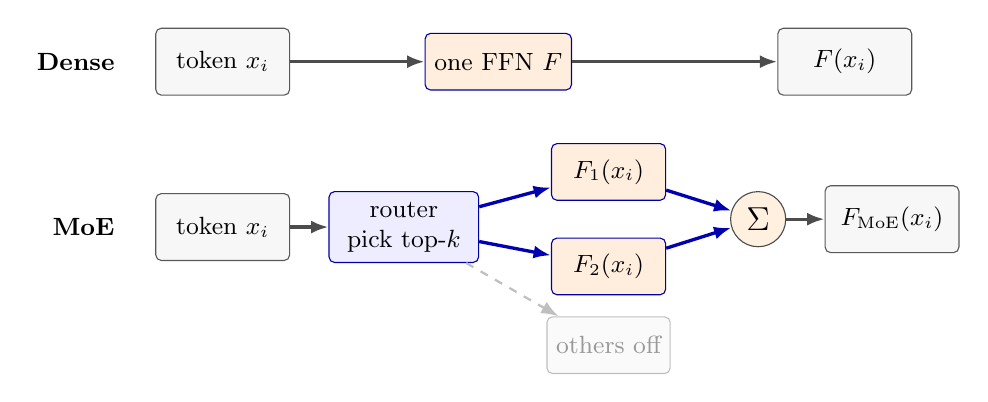
\begin{tikzpicture}[
    >={Latex[length=2.2mm]},
    flow/.style={->,very thick,draw=black!70},
    chosen/.style={->,very thick,draw=blue!70!black},
    unused/.style={->,thick,dashed,draw=black!25},
    box/.style={draw=black!65,fill=black!3,rounded corners=2pt,
      minimum width=1.7cm,minimum height=0.85cm,align=center,font=\small},
    router/.style={draw=blue!65!black,fill=blue!7,rounded corners=2pt,
      minimum width=1.9cm,minimum height=0.9cm,align=center,font=\small},
    expert/.style={draw=blue!65!black,fill=orange!13,rounded corners=2pt,
      minimum width=1.45cm,minimum height=0.72cm,align=center,font=\small},
    muted/.style={draw=black!25,fill=black!2,text=black!40,rounded corners=2pt,
      minimum width=1.45cm,minimum height=0.72cm,align=center,font=\small},
    add/.style={circle,draw=black!70,fill=orange!12,minimum size=7mm,
      inner sep=0pt,font=\large},
    rowlabel/.style={font=\bfseries\small,anchor=east}
  ]
    \node[rowlabel] at (-0.55,1.55) {Dense};
    \node[box] (xd) at (0.7,1.55) {token $x_i$};
    \node[expert] (fd) at (4.2,1.55) {one FFN $F$};
    \node[box] (yd) at (8.6,1.55) {$F(x_i)$};
    \draw[flow] (xd) -- (fd);
    \draw[flow] (fd) -- (yd);

    \node[rowlabel] at (-0.55,-0.55) {MoE};
    \node[box] (xm) at (0.7,-0.55) {token $x_i$};
    \node[router] (r) at (3.0,-0.55) {router\\pick top-$k$};
    \node[expert] (f1) at (5.6,0.15) {$F_1(x_i)$};
    \node[expert] (f2) at (5.6,-1.05) {$F_2(x_i)$};
    \node[muted] (off) at (5.6,-2.05) {others off};
    \node[add] (sum) at (7.5,-0.45) {$\Sigma$};
    \node[box] (ym) at (9.2,-0.45) {$F_{\mathrm{MoE}}(x_i)$};
    \draw[flow] (xm) -- (r);
    \draw[chosen] (r) -- (f1);
    \draw[chosen] (r) -- (f2);
    \draw[unused] (r) -- (off);
    \draw[chosen] (f1) -- (sum);
    \draw[chosen] (f2) -- (sum);
    \draw[flow] (sum) -- (ym);
  \end{tikzpicture}%
  }
  \caption{A dense FFN uses the same parameters for every token.  An MoE layer
  chooses a small subset of experts and combines only their outputs.}
  \label{fig:dense-versus-moe}
\end{figure}

\subsection{What one expert computes}

One expert is the entire FFN map $F_e$ in
Equation~\eqref{eq:moe-expert}.  Its three matrices
$W_{\mathrm{gate}}^{(e)}$, $W_{\mathrm{up}}^{(e)}$, and
$W_{\mathrm{down}}^{(e)}$ all belong to expert $e$.  This document uses a
SwiGLU FFN: its gate path and content path are multiplied componentwise, then
projected back to the residual width:
\begin{equation}
  F_e(x)
  =W_{\mathrm{down}}^{(e)}
   \left[
     \SiLU\!\left(W_{\mathrm{gate}}^{(e)}x\right)
     \odot
     \left(W_{\mathrm{up}}^{(e)}x\right)
   \right].
  \label{eq:moe-expert}
\end{equation}

\begin{figure}[H]
  \centering
  \resizebox{0.96\linewidth}{!}{%
  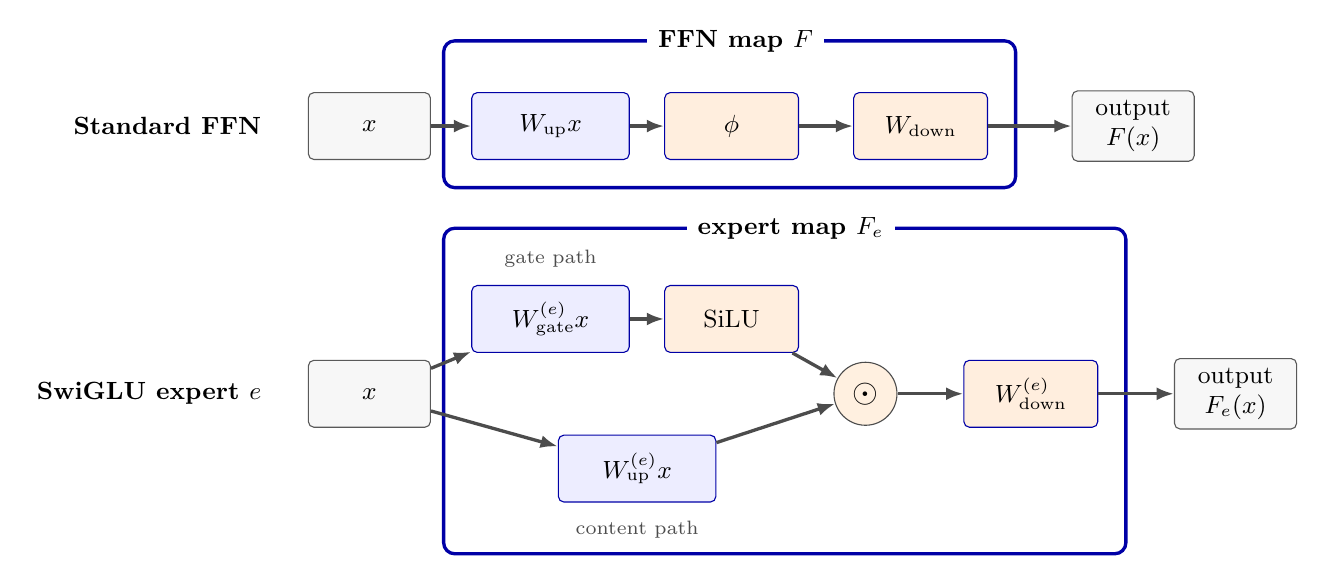
\begin{tikzpicture}[
    >={Latex[length=2.2mm]},
    flow/.style={->,very thick,draw=black!70},
    branch/.style={draw=blue!65!black,fill=blue!7,rounded corners=2pt,
      minimum width=2.0cm,minimum height=0.85cm,align=center,font=\small},
    operation/.style={draw=blue!65!black,fill=orange!13,rounded corners=2pt,
      minimum width=1.7cm,minimum height=0.85cm,align=center,font=\small},
    tensor/.style={draw=black!65,fill=black!3,rounded corners=2pt,
      minimum width=1.55cm,minimum height=0.85cm,align=center,font=\small},
    mapbox/.style={draw=blue!65!black,very thick,rounded corners=4pt},
    maplabel/.style={font=\bfseries\small,fill=white,
      inner xsep=4pt,inner ysep=1pt},
    multiply/.style={circle,draw=black!70,fill=orange!12,minimum size=8mm,
      inner sep=0pt,font=\large},
    note/.style={font=\scriptsize,text=black!70,align=center},
    rowlabel/.style={font=\bfseries\small,anchor=east,align=right}
  ]
    % Standard dense FFN: one hidden path.
    \node[rowlabel] at (-0.45,2.4) {Standard FFN};
    \node[tensor] (xd) at (0.8,2.4) {$x$};
    \node[branch] (upd) at (3.1,2.4) {$W_{\mathrm{up}}x$};
    \node[operation] (actd) at (5.4,2.4) {$\phi$};
    \node[operation] (downd) at (7.8,2.4) {$W_{\mathrm{down}}$};
    \node[tensor] (outd) at (10.5,2.4) {output\\$F(x)$};
    \draw[mapbox]
      ($(upd.north west)+(-0.35,0.65)$) rectangle
      ($(downd.south east)+(0.35,-0.35)$);
    \node[maplabel] at (5.45,3.475) {FFN map $F$};
    \draw[flow] (xd) -- (upd);
    \draw[flow] (upd) -- (actd);
    \draw[flow] (actd) -- (downd);
    \draw[flow] (downd) -- (outd);

    % SwiGLU expert: content and gate paths.
    \node[rowlabel] at (-0.45,-1.0) {SwiGLU expert $e$};
    \node[tensor] (xe) at (0.8,-1.0) {$x$};
    \node[branch] (gate) at (3.1,-0.05) {$W_{\mathrm{gate}}^{(e)}x$};
    \node[operation] (silu) at (5.4,-0.05) {$\SiLU$};
    \node[branch] (up) at (4.2,-1.95) {$W_{\mathrm{up}}^{(e)}x$};
    \node[multiply] (mul) at (7.1,-1.0) {$\odot$};
    \node[operation] (down) at (9.2,-1.0) {$W_{\mathrm{down}}^{(e)}$};
    \node[tensor] (out) at (11.8,-1.0) {output\\$F_e(x)$};
    \draw[mapbox]
      ($(gate.north west)+(-0.35,0.72)$) rectangle
      ($(down.south east)+(0.35,-1.60)$);
    \node[maplabel] at (6.15,1.095) {expert map $F_e$};
    \draw[flow] (xe) -- (gate);
    \draw[flow] (xe) -- (up);
    \draw[flow] (gate) -- (silu);
    \draw[flow] (silu) -- (mul);
    \draw[flow] (up) -- (mul);
    \draw[flow] (mul) -- (down);
    \draw[flow] (down) -- (out);
    \node[note,above=3pt of gate] {gate path};
    \node[note,below=3pt of up] {content path};
  \end{tikzpicture}%
  }
  \caption{The outlined boxes are the complete maps.  The lower box---not its
  final arrow---is the expert $F_e$ defined by
  Equation~\eqref{eq:moe-expert}; $F_e(x)$ is its output.}
  \label{fig:swiglu-expert}
\end{figure}

The superscript $(e)$ means that every expert has its own three projection
matrices.  MoE changes only which expert receives the token; it does not change
the expert itself or the attention layer
\citep{shazeer2020glu,lepikhin2020gshard}.

\subsection{How the router picks experts}

The mainstream design is \emph{token-choice top-$k$ routing}: each token scores
all experts and chooses its own winners.  Expert-choice routing, global matching,
hash routing, and reinforcement-learning routers exist, but they are not the
standard path in current large language models
\citep{hashimoto2026attentionmoe}.

In this section, $i$ always indexes tokens and $e$ always indexes experts.  For
token vector $x_i\in\R^{d_{\mathrm{model}}}$, the router produces one score per
expert:
\begin{equation}
  r_i=W_rx_i\in\R^E,
  \qquad
  W_r\in\R^{E\times d_{\mathrm{model}}}.
  \label{eq:moe-router}
\end{equation}
The $k$ largest scores determine the selected expert set
\begin{equation}
  \mathcal{S}_i=\TopK(r_i,k).
  \label{eq:moe-selection}
\end{equation}
For selected-softmax routing, softmax over those selected scores gives their
mixing weights:
\begin{equation}
  g_{i,e}
  =\frac{\exp(r_{i,e})}
         {\sum_{e'\in\mathcal{S}_i}\exp(r_{i,e'})},
  \qquad e\in\mathcal{S}_i.
  \label{eq:moe-gates}
\end{equation}
Finally, run the selected experts and add their weighted outputs:
\begin{equation}
  F_{\mathrm{MoE}}(x_i)
  =\sum_{e\in\mathcal{S}_i}g_{i,e}F_e(x_i).
  \label{eq:moe-output}
\end{equation}
That is the complete MoE computation.

\begin{figure}[H]
  \centering
  \resizebox{0.97\linewidth}{!}{%
  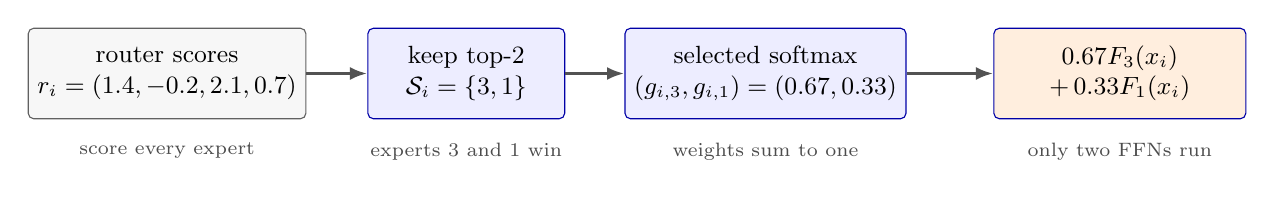
\begin{tikzpicture}[
    >={Latex[length=2.2mm]},
    arrow/.style={->,very thick,draw=black!68},
    stagebox/.style={draw=black!62,fill=black!3,rounded corners=2pt,
      minimum width=2.5cm,minimum height=1.15cm,align=center,font=\small},
    select/.style={draw=blue!65!black,fill=blue!7,rounded corners=2pt,
      minimum width=2.5cm,minimum height=1.15cm,align=center,font=\small},
    result/.style={draw=blue!65!black,fill=orange!13,rounded corners=2pt,
      minimum width=3.2cm,minimum height=1.15cm,align=center,font=\small},
    note/.style={font=\scriptsize,text=black!70}
  ]
    \node[stagebox] (scores) at (0,0)
      {router scores\\$r_i=(1.4,-0.2,2.1,0.7)$};
    \node[select] (top) at (3.8,0)
      {keep top-$2$\\$\mathcal{S}_i=\{3,1\}$};
    \node[select] (weights) at (7.6,0)
      {selected softmax\\$(g_{i,3},g_{i,1})=(0.67,0.33)$};
    \node[result] (out) at (12.1,0)
      {$0.67F_3(x_i)$\\$+\,0.33F_1(x_i)$};
    \draw[arrow] (scores) -- (top);
    \draw[arrow] (top) -- (weights);
    \draw[arrow] (weights) -- (out);
    \node[note,below=5pt of scores] {score every expert};
    \node[note,below=5pt of top] {experts $3$ and $1$ win};
    \node[note,below=5pt of weights] {weights sum to one};
    \node[note,below=5pt of out] {only two FFNs run};
  \end{tikzpicture}%
  }
  \caption{A concrete top-$2$ routing example with four experts.}
  \label{fig:moe-topk-example}
\end{figure}

The most common variants differ only in how many winners are kept and how their
weights are formed:

\begin{center}
\small
\begin{tabularx}{\textwidth}{@{}>{\raggedright\arraybackslash}p{0.24\textwidth} X X@{}}
\toprule
Router & Selection and weights & Main trade-off \\
\midrule
Top-$1$ token choice \citep{fedus2022switch}
  & Keep one softmax winner.
  & Minimal expert compute and communication; most sensitive to imbalance. \\
Top-$k$ selected softmax \citep{jiang2024mixtral}
  & Keep a few logits, then normalize the selected logits as in
    Equations~\eqref{eq:moe-selection}--\eqref{eq:moe-gates}.
  & More robust mixtures at the cost of running multiple experts. \\
Sigmoid top-$k$ with load bias \citep{deepseekai2024deepseekv3}
  & Rank sigmoid scores after adding per-expert selection biases.
  & Separates routing balance from mixture weights; requires online bias updates. \\
\bottomrule
\end{tabularx}
\end{center}

Across these variants, the core remains \emph{score, select, run, combine}.

\subsection{How an MoE is trained}

An MoE uses the same next-token loss as a dense Transformer.  Routing changes
which parameters receive that loss.

Top-$k$ selection has no derivative.  For token $i$, hold the selected set
$\mathcal{S}_i$ fixed during backpropagation.  The language-model loss then
updates the selected experts.  Equation~\eqref{eq:moe-gates} updates relative
router scores only for $k>1$.  Switch top-$1$ instead retains the selected
expert's full-softmax probability as its gate, so the router still receives a
gradient.  The next
forward pass computes top-$k$ again from the updated scores, so the selected set
can change.  Experts outside $\mathcal{S}_i$ receive no gradient from $x_i$.

Two router problems require extra control.  The first is expert collapse: a few
experts receive most tokens.  The second is large raw router scores.  These
scores are the logits $r_{i,e}$.  Softmax cannot see a common offset:
\[
  \softmax(r_i+c\mathbf{1})=\softmax(r_i).
\]
The offset $c$ can therefore drift without changing the routing probabilities.
Large positive offsets reduce numerical headroom in low-precision training.  A
standard $z$-loss penalizes the router log-partition:
\begin{equation}
  \mathcal{L}_z
  =\frac{1}{T}\sum_{i=1}^{T}
    \left[\log\!\left(\sum_{e=1}^{E}\exp(r_{i,e})\right)\right]^2.
  \label{eq:moe-z-loss}
\end{equation}
Inside the sum, the exponential makes the loss sensitive to large router
scores: the largest scores rapidly dominate the sum.  The outer logarithm then
brings the result back from exponential scale to the scale of the router
scores.  The loss therefore reacts strongly to an excessively large score
without itself spanning the enormous range of the raw exponential sum.

The reason for balancing is easiest to see before top-$k$ selection.  Let
$p_{i,e}$ be the router probability for expert $e$, and average it over the
tokens:
\begin{equation}
  p_{i,e}=\softmax(r_i)_e,
  \qquad
  \bar p_e=\frac{1}{T}\sum_{i=1}^{T}p_{i,e}.
  \label{eq:moe-mean-router-probability}
\end{equation}
The vector $\bar p$ describes how the batch is distributed across experts.  To
spread that distribution, maximize its entropy, or equivalently minimize
\begin{equation}
  \mathcal{L}_{\mathrm{ent}}
  =\sum_{e=1}^{E}\bar p_e\log \bar p_e.
  \label{eq:moe-routing-entropy}
\end{equation}
Its minimum is the uniform distribution, $\bar p_e=1/E$.  The entropy is taken
over the batch average $\bar p$, not over each token's distribution $p_i$.
Individual routing decisions can therefore remain sharp.  Even so, maximum
entropy makes a perfectly even batch distribution the target.  That is stronger
than necessary: experts may receive unequal traffic as they specialize.  The
practical goal is only to prevent a few experts from receiving an unusually
large share.

The implementation therefore measures the experts actually selected by
top-$k$.  Their assignment frequencies are
\begin{equation}
  f_e=\frac{1}{Tk}\sum_{i=1}^{T}\mathbf{1}\!\left[e\in\mathcal{S}_i\right].
  \label{eq:moe-load-statistics}
\end{equation}
Thus $f_e$ supplies the actual selection frequency that is missing from the soft
probability distribution $\bar p$.  Because top-$k$ selection is discrete,
$f_e$ is treated as fixed during backpropagation.  A common load-aware penalty is
\begin{equation}
  \mathcal{L}_{\mathrm{bal}}
  =E\sum_{e=1}^{E}f_e\bar p_e.
  \label{eq:moe-balance-loss}
\end{equation}
When the hard assignment frequencies follow the mean probabilities,
$f_e\approx\bar p_e$, this behaves like $E\sum_e\bar p_e^2$: a quadratic penalty
for a concentrated distribution.  Its formal minimum is also uniform, but
large components dominate the quadratic penalty while small components
contribute little.  With a small coefficient $\alpha$, it therefore acts mainly
against unusually large expert usage rather than enforcing a perfectly even
distribution.  The factors remain separate because $f_e$ measures the actual
discrete load, while $\bar p_e$ supplies the gradient to the router
\citep{fedus2022switch,qiu2025loadbalancing,hashimoto2026attentionmoe}.

With both auxiliary losses defined, the full objective is
\begin{equation}
  \mathcal{L}
  =\mathcal{L}_{\mathrm{LM}}
   +\alpha\mathcal{L}_{\mathrm{bal}}
   +\beta\mathcal{L}_{z},
  \label{eq:moe-training-loss}
\end{equation}
Here, $\mathcal{L}_{\mathrm{LM}}$ is the usual cross-entropy loss.  The
coefficients $\alpha$ and $\beta$ control the strengths of the balance loss and
the $z$-loss.

\section{Linear Attention and RNN}

Coming soon.

\bibliographystyle{plainnat}
\bibliography{references}

\end{document}
